\selectlanguage{australian}%

\chapter{\label{chap:Literature-Review}Literature Review}

\acresetall

This literature review aims to outline some of the key concepts involved
in this thesis, and to summarise progress on similar endeavours made
thus far.


\section{Babble and other Speech-Related Noise}

In signal analysis, noise is defined as an unwanted signal. In acoustics,
a wide range of types of noise may interfere with a signal. This noise
originates from somewhere within the environment: from a stationary
source, or a non-stationary source. Generally this noise is additive,
meaning the mixed signal can be considered as the desired signal plus
noise.

In this thesis the desired signal, or \acf{SoI} signal, is considered
to be a speech signal and the additive noise signal (or masker) is
considered to be a number of competing speech signals. Noise originating
from speakers can be classified by the number of speakers as \acf{SSN},
babble noise or competing speaker noise, as defined in \tabref{Speech-related-noise-types}.

\begin{table}[h]
\centering{}\protect\caption{Speech-related noise types\label{tab:Speech-related-noise-types}}
\begin{tabular*}{1\textwidth}{@{\extracolsep{\fill}}|p{0.25\textwidth}|p{0.45\textwidth}|p{0.2\textwidth}|}
\hline 
\textbf{Type of Speech-Related Noise} & \textbf{Definition \citep{Krishnamurthy2009}} & \textbf{Steady-State or Time-Varying}\tabularnewline
\hline 
\ac{SSN} & A diffused background rumble, where individual conversations or speakers
are not distinguishable. & Steady-state\tabularnewline
\hline 
Babble Noise & Individual speakers can be heard and at times, individual words can
also be heard. & Time-varying\tabularnewline
\hline 
Competing Speaker & There are two speakers present. & Time-varying\tabularnewline
\hline 
\end{tabular*}
\end{table}


Babble noise is often considered the most difficult noise condition
for speech processing due to the fact it is very similar in structure
to the desired clean signal, and due to the time-variant structure
(unlike \ac{SSN}) \citep{Krishnamurthy2009}.

The exact distinction between babble and \ac{SSN} is under-defined
and subjective. \tabref{Subjective-classification-noise} below shows
test results by \citet{Krishnamurthy2009} where subjects were asked
to listen to a recording of a number of speakers and classify whether
they could identify individual speakers. It was found that for four
to six speakers the classification of whether noise was babble or
speech-shaped varied from person-to-person, even for the same recording.

\begin{table}[h]
\protect\caption{Subjective classification of babble noise vs. \acl{SSN}\label{tab:Subjective-classification-noise}}
\begin{tabular*}{1\textwidth}{@{\extracolsep{\fill}}|>{\centering}p{0.3\textwidth}|>{\centering}p{0.3\textwidth}|>{\centering}p{0.3\textwidth}|}
\hline 
\textbf{Number of Speaker in Babble} & \textbf{Percentage of Speakers Identifying Recording as Babble} & \textbf{Percentage of Speakers Identifying Recording as Speech-Shaped}\tabularnewline
\hline 
$\leq3$ & 100\% & 0\%\tabularnewline
\hline 
4 & 66\% & 34\%\tabularnewline
\hline 
5 & 18\% & 82\%\tabularnewline
\hline 
6 & 27\% & 73\%\tabularnewline
\hline 
$\geq7$ & 0\% & 100\%\tabularnewline
\hline 
\end{tabular*}
\end{table}


Human listeners compensate for babble and competing speaker noise
by exploiting the time-modulated property of the noise. Listeners
focus on the target speech during moments of low noise levels to piece
together the target\textquoteright s message. Therefore, human recognition
in modulated noise is better than in steady-state noise. However,
the opposite is true for a machine: steady state noise conditions
are easier to handle than modulated noise with \ac{DSP} techniques
\citep{Loizou2013a}. Of course, the level of improvement directly
depends on the speech enhancement technique used.


\section{Speech Enhancement}

Speech enhancement has various practical applications, including:
\begin{itemize}
\item improving hearing with hearing aids and cochlear implants \citep{Wang2008,Yang2005},
\item increasing the accuracy of ASR systems,
\item denoising of telecommunications systems
\item and refining recorded audio \citep{Benesty2005}.
\end{itemize}
Due to the many application areas, various algorithms may be used
under different contexts in order to balance the condition-specific
performance, calculation efficiency, flexibility and ease of implementation.
\figref{Speech-Enhance-Classifications} \vpageref{fig:Speech-Enhance-Classifications}
illustrates some of the many variations in methods for speech enhancement,
with data extracted from \citep{Yang2005,Pollack1958,Loizou2013b,Kamath2002}.
Some methods provide better performance than others, but at the expense
of practicality. For example, recognition can be improved under non-stationary
noise by using a microphone array, however such a set up is more expensive.

\begin{figure}[p]
\centering{}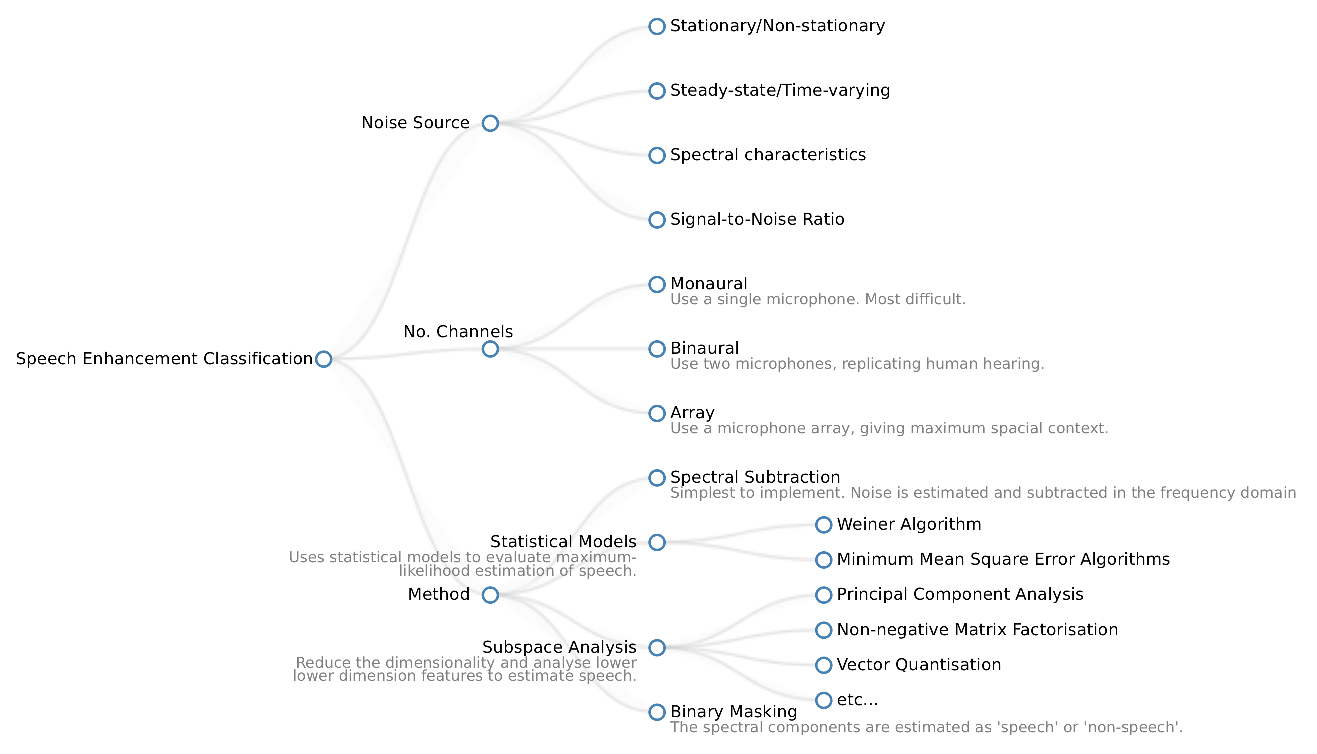
\includegraphics[angle=90,height=0.9\textheight]{fig/speech-enhancement-methods}\protect\caption{Some classifications of Speech Enhancement Methods\label{fig:Speech-Enhance-Classifications}}
\end{figure}



\section{Modelling Babble}

In a multi-speaker environment, and ignoring other forms of noise,
a signal can be considered a sum of multiple speakers:

\begin{equation}
X_{Babble}=\sum X_{Speakers}\label{eq:babble-sum-speakers}
\end{equation}


\nomenclature{$X$}{Short-time Fourier transform of a signal or recording, either with or without noise present. Rows represent frequency bins and columns represent time frames.}

(\ref{eq:babble-sum-speakers}) follows directly from the definition
of babble. The number of speaker signals used may vary, but to align
with with the definition for babble should be between three and six.


\subsection{For Generation}

It is generally desirable in testing to be able to present noise at
different \acp{SNR}. Rather than recording noise in a range of conditions
directly, it is more convenient to have separate speech and noise
and to model the speech with noise signal. Thus, the effects of babble
are often modelled rather than directly recorded. This type of babble
can be classed as synthetic babble, and may or may not accurately
represent real babble \citep{Krishnamurthy2009}.

The most common method of creating synthetic babble is to use a number
of speech recordings, adding them together to form babble. This presents
a number of issues. Firstly, real conversations are not simply a number
of voices speaking simultaneously. Rather, conversations are dynamic,
where there is generally one speaker but occasionally more or none
\citep{Krishnamurthy2009}. Secondly, synthetic babble generally does
not take into effect environmental effects, such as reverberation,
generally present alongside babble \citep{Krishnamurthy2009}.


\subsection{For Analysis and Enhancement}

For analysis, it is generally preferable to model a signal as a sum
consisting of a desired component and a noise component. The babble
model may exploit (\ref{eq:babble-sum-speakers}), such that a single
voice is modelled and extended to multiple speakers \citep{Mohammadiha2013a},
whereas other methods leave the model for babble as a generic noise
model \citep{Wilson2008}. The advantage of the latter is that the
same model may be applicable to other forms of noise.


\subsection{Separating Speech from Babble}

When the cocktail party problem was originally proposed, five factors
were identified as to how the human brain may differentiate between
the sources \citep{Cherry1953}, shown in \figref{Differentiating-Speech-Babble}
\vpageref{fig:Differentiating-Speech-Babble}.

\begin{figure}[h]
\centering{}\includegraphics[width=1\textwidth]{\string"fig/babble Separation\string".eps}\protect\caption{Differentiating Speech from Babble\label{fig:Differentiating-Speech-Babble}}
\end{figure}


Algorithms taking advantage of spatial differences and visual cues,
although effective \citep{Dupont2000}, require multiple channels
and visual data. Subspace methods take advantage of differences in
voices and differences in pronunciation. \ac{HMM} models for speech
recognition also take advantage of transitional probabilities \citep{Mohammadiha2013}.


\section{Methods for Evaluation of Speech Enhancement}

Methods for evaluating the intelligibility of speech, and by extension
speech enhancement, can be classified by the type of recognition they
measure: \ac{ASR} vs. \ac{HR}. This is necessary since \ac{ASR}
systems often recognise speech through a relatively low dimension
feature vector, whereas the human brain is far more sensitive. An
algorithm for enhancement may indeed improve the intelligibility for
an \ac{ASR} system, but side effects may be distracting or distortive
to a human listener.


\subsection{Human Recognition}

Intelligibility of a speech signal by humans is difficult to accurately
and quantitatively measure. The most obvious measure is to have human
test subjects listen to signals and judge which are more intelligible.
In order to achieve reputable, repeatable and accurate results a large
test is required with a large number of test subjects and recordings.

The \ac{ITU} standard for such tests is the \ac{MOS} \citep{InternationalTelecommunicationUnion1996}.
The test is designed to give an indication of the quality of telecommunication
transmission, but is applicable as a measure of speech intelligibility.
The \ac{MOS} results are a score calculated by the mean of the listeners\textquoteright{}
scores in the range one to five, with one representing the worst quality
and five representing the highest quality of intelligibility.

\ac{PESQ} is the \ac{ITU} standard for evaluation of objective speech
quality \citep{Rix2001,InternationalTelecommunicationUnion2001}.
This method provides an algorithm which estimates the improvement
quality by comparing a system\textquoteright s input and output \citep{Rix2001}.
Results show \ac{PESQ} scores give consistent and reliable estimates
on human perception, although are not directly comparable with \ac{MOS}
scores \citep{Rix2003}. Other methods for measuring perceptual quality
include long-term \ac{SNR}, segmental \ac{SNR}, weighted spectral
slope, log-likelihood ratio, Itakura-Saito distance, cepstrum distance,
\ac{SD}, \ac{SDR} and variations \citep{Hu2008}.


\subsection{Machine Recognition}

The most common technique to evaluate machine recognition quality
of speech is to run an \ac{ASR} algorithm on the signal and perform
a comparison of the \ac{WRR}. It should be noted that this method
is somewhat limited, in that different \ac{ASR} algorithms, which
may implement different feature vectors, may perform differently.
As such, results from different \ac{ASR} algorithms are not directly
comparable.

Algorithms in literature tend to limit evaluation methods to either
human recognition or machine recognition methods, as seen in \figref{Assessment-methods},
showing the evaluation measures used in various papers. This data
was gathered from the following papers \citep{Mohammadiha2013a,Wilson2008,Schmidt2006,Raj2005,Raj2005a,Raj2011,Fevotte2011}.

\begin{figure}[h]
\selectlanguage{english}%


\selectlanguage{australian}%
\centering{}\includegraphics[width=1\textwidth]{\string"fig/assessment Methods\string".eps}\protect\caption{Assessment methods used in literature\label{fig:Assessment-methods}}
\end{figure}



\section{Subspace Methods by Decomposition}

Subspace methods focus on reducing the dimensionality of a system.
This is done by decomposition or factorisation of a signal into lower
dimensional systems. Many techniques exist for decomposing a signal,
some of which are outlined in \figref{subspace-decomposition}.

\begin{figure}[H]
\selectlanguage{english}%


\selectlanguage{australian}%
\centering{}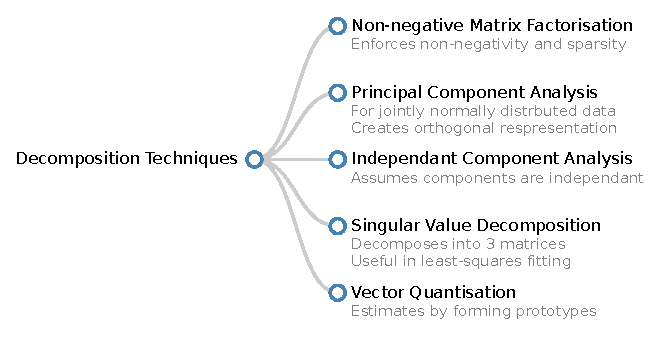
\includegraphics{fig/subspace}\protect\caption{Mathematical decomposition techniques for subspace analysis\label{fig:subspace-decomposition}}
\end{figure}


These techniques factorise a matrix into two matrix factors of the
form:

\[
C_{i\times j}\approx B_{i\times k}A_{k\times j}
\]


\nomenclature{$i$, $j$, $k$}{Matrix indexing placeholders.}

Often $k\ll i$ and $k\ll j$, meaning the factorised form may be
considered a more compact form.

\acf{NMF}, previously known as positive matrix factorisation, was
popularised by \citet{Lee1999} as a method lending itself to breaking
objects into their composing parts The distinguishing characteristic
of \ac{NMF} is that the product matrix, along with both its factors,
are non-negative, i.e. $A_{ij}\ge0,\, B_{ij}\ge0,\, C_{ij}\ge0\quad\forall\, i,\, j$.
\ac{NMF} has been demonstrated to be an effective method in dividing
images into parts \citep{Lee1999,Donoho2003}. Furthermore, \ac{NMF}
also has been shown to be useful on signals, specifically as a source-
separation algorithm \citep{Mohammadiha2013a,Wilson2008,Mohammadiha2013}.


\subsection{\acl{NMF} and Speech}

\ac{NMF} can be used in signal analysis, such that \citep{Lee1999,Paatero1994}:

\begin{equation}
X_{n_{f}\times n_{s}}\approx V_{n_{f}\times n_{c}}W_{n_{c}\times n_{s}}\label{eq:nmf-approx}
\end{equation}


where:
\begin{itemize}
\item $X$ represents the signal with rows of frequency bins results from
a Fourier transform and columns of time segments;
\item $V$ is the spectral components with columns representing typical
spectral vectors;
\item $W$ is the activation matrix, where each row represents the activation
levels of components at given times;
\item $n_{f}$ is the number of Frequency bins;
\item $n_{s}$ is the number of samples; and
\item $n_{c}$ is the number of components.
\end{itemize}
\nomenclature{$V$}{Spectral component matrix, one of the decompositions formed through the non-negative matrix factorisation procedure. Rows represent frequency bins and columns represent the component bases.}\nomenclature{$W$}{Activation matrix, one of the decompositions formed through the non-negative matrix factorisation procedure. Rows represent the component bases and columns represent time frames.}\nomenclature{$n_f$}{The total number of frequency bins.}\nomenclature{$n_s$}{The total number of time frames (samples).}\nomenclature{$n_c$}{The total number of component bases.}

\figref{nmf-on-speech} \citep{Mohammadiha2013} shows a visual representation
of this factorisation. It can be seen that the columns of the spectral
component matrix, $V$, represent approximations of the spectral components,
and that the activation matrix, $W$, is sparse.

\begin{figure}[h]
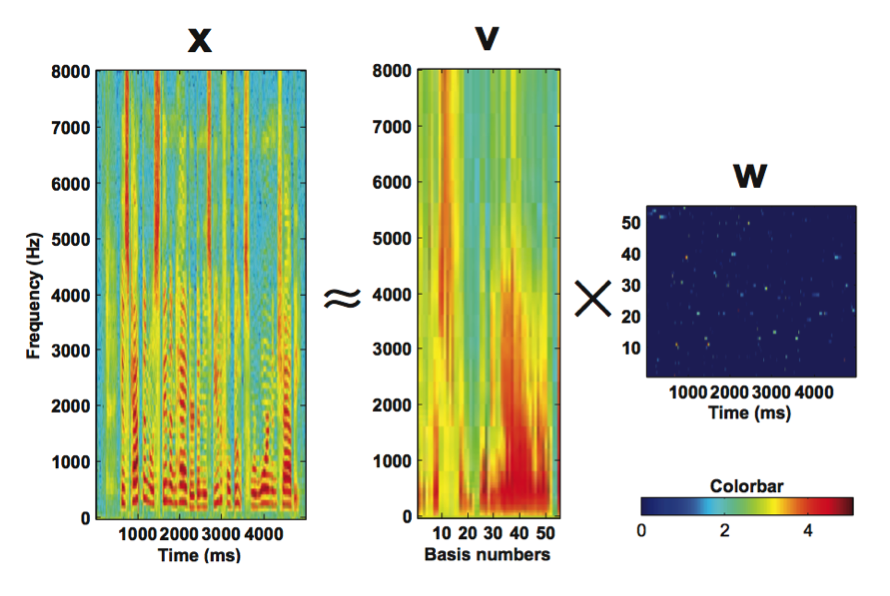
\includegraphics[width=1\textwidth]{fig/NMF-speech}\protect\caption{\acl{NMF} on speech\label{fig:nmf-on-speech}}
\end{figure}



\section{Assessment of Methods of Factorisation}


\subsection{Objective Functions}

\ac{NMF} algorithms aim to minimise or maximise an objective function.
The objective function is designed with an intent that optimisation
will ensure the approximation in (\ref{eq:nmf-approx}). The common
choice is to minimise the square error, or Euclidean distance between
$X$ and $VW$ seen in (\ref{eq:euclidean-distance-def}) \citep{Lee2000}.

\begin{equation}
F=\left\Vert X-VW\right\Vert ^{2}=\sum_{f=1}^{n_{f}}\sum_{s=1}^{n_{s}}\left[X_{fs}-\left(VW\right)_{fs}\right]^{2}\label{eq:euclidean-distance-def}
\end{equation}


\nomenclature{$F$}{The chosen objective function.}\nomenclature{$\Vert . \Vert ^2$}{Indicates the Euclidean distance.}\nomenclature{$f$}{Frequency bin index.}\nomenclature{$s$}{Time frame (sample) index.}

Another standard objective function based on the Kullback-Leibler
divergence of $VW$ from $X$ was proposed by \citet{Lee1999} and
is given as (\ref{eq:kl-divergence-def}). Here, the objective is
maximisation of the divergence objective function.

\begin{equation}
F=D_{KL}\left(X\|VW\right)=\sum_{f=1}^{n_{f}}\sum_{s=1}^{n_{s}}\left[X_{fs}\log\left(VW\right)_{fs}-\left(VW\right)_{fs}\right]\label{eq:kl-divergence-def}
\end{equation}


\nomenclature{$D_{KL}\left(.\right)$}{Indicates the Kullback-Leibler divergence.}

Often a modified objective function is used. This may add a cost function
in order to achieve auxiliary constraints \citep{Berry2007}. Some
examples of this are further discussed below. The objective function
is implemented using a series of update functions. The update functions
are iteratively processed until the approximation of $VW$ to $X$
is sufficient.


\subsection{Multiplicative Update Algorithms\label{sub:Multiplicative-Update-Algorithms}}

Updates are often implemented multiplicatively, since if all initial
matrices are non-negative and multiplications are positive, then the
final matrix will also implicitly be non-negative. This prevents the
need to explicitly enforce non-negativity. For the Euclidean distance
objective function, the multiplicative update rules are \citep{Lee2000}:

\begin{equation}
V_{fc}\leftarrow V_{fc}\otimes\left(XW^{T}\right)\oslash\left(VWW^{T}\right)\label{eq:mult-update-euc-v}
\end{equation}


\nomenclature{$\leftarrow$}{Indicates an iterative update rule.}\nomenclature{$\otimes$}{Element-wise multiplication.}\nomenclature{$\oslash$}{Element-wise division.}\nomenclature{$\left(.\right)^T$}{Matrix transpose.}\nomenclature{$c$}{Component base index.}

and:

\begin{equation}
W_{cs}\leftarrow W_{cs}\otimes\left(V^{T}X\right)\oslash\left(V^{T}VW\right)\label{eq:mult-update-euc-w}
\end{equation}


where $\otimes$ and $\oslash$ are the element-wise multiplication
and division operators. Alternatively, if the divergence objective
function is to be used,

\begin{equation}
V_{fc}\leftarrow V_{fc}\sum_{s}\frac{X_{fs}}{\left(VW\right)_{fs}}W_{cs}\label{eq:mult-update-div-v}
\end{equation}


and:

\begin{equation}
W_{cs}\leftarrow W_{cs}\sum_{s}V_{fc}\frac{X_{fs}}{(VW)_{fs}}\label{eq:mult-update-div-w}
\end{equation}


provide the required update rules \citep{Lee1999}. Additionally,
a third update rule \citep{Lee1999}:

\begin{equation}
V_{fs}\leftarrow\frac{V_{fc}}{\sum_{f}V_{fc}}\label{eq:mult-update-div-normalise}
\end{equation}


was included to normalise columns in the component matrix. This is
included to prevent continuously updating $V$ by a constant and $W$
by its inverse, which would otherwise be a valid update since $VW$
would be identical.

In addition, equivalent additive expressions can be formulated, known
as the gradient descent algorithms \citep{Lee2000,Berry2007}. In
this thesis, these forms are considered as equivalent \citep{Berry2007}
and thus are not considered separately.

The multiplicative update method of \ac{NMF} has been used extensively
in literature with good results \citep{Wilson2008,Raj2005}. However,
it has been shown that the proof given by \citet{Lee2000}, attempting
to prove the convergence of the multiplicative update rules (\ref{eq:mult-update-euc-v})
through (\ref{eq:mult-update-div-normalise}), was incomplete \citep{Berry2007,Finesso2006}.
The above equations may become stuck at stationary points and do not
always converge to the desired objective function \citep{Berry2007,Finesso2006,Finesso2004}.
When an element in $V$ or $W$ becomes zero it becomes \textquotedblleft locked\textquotedblright{}
and must remain as zero, an inherent flaw of the multiplicative update
functions \citep{Albright2006}. The following class of algorithms
allow flexibility in this respect.


\subsection{\acl{ALS} Algorithms}

\ac{ALS} algorithms are based on the initial proposed algorithms
by \citet{Paatero1994}. These algorithms are based on the alternating
variables method (or coordinate descent method) \citep{Wright1999}.
In these algorithms, first $V$ is fixed and $W$ is calculated using
a least squares method, then $W$ is fixed and $V$ is calculated
in a similar manner. These two steps are repeated until an adequate
approximation is achieved \citep{Albright2006}.

The least squares method used varies between \ac{ALS} algorithms.
\ac{ALS} algorithms can be generally classified by whether a non-negative
least squares method is used; or a general least squares method where
any negative values are subsequently set to zero. Non-negative least
squares methods converge to a local minimum successfully, however
the calculation cost per iteration is far higher despite attempts
to improve performance \citep{Berry2007,Albright2006,Lin2007,VanBenthem2004,Bro1997}.
General least squares methods may converge to a saddle point as opposed
to a minima. This is generally still preferred under practical conditions
due to the speed. Performance can also be improved by using a good
initialisation.

Typical \ac{ALS} algorithms \citep{Berry2007} using general least
squares method resemble the following:
\begin{enumerate}
\item Initialise $V$
\item Repeat the following for a predefined number of iterations:

\begin{enumerate}
\item Solve for $W$ using (\ref{eq:als-update-w}).
\item Set any negative elements in $W$ to zero.
\item Solve for $V$ using (\ref{eq:als-update-v}).
\item Set any negative elements in $V$ to zero.
\end{enumerate}
\end{enumerate}
\begin{equation}
V^{T}VW=V^{T}X\label{eq:als-update-w}
\end{equation}


\begin{equation}
WW^{T}V^{T}=WX^{T}\label{eq:als-update-v}
\end{equation}


The algorithms presented thus far present a common weakness in that
the update rules for the component matrix and the activation matrix
are the same (except that in some cases the component matrix also
has a normalisation update). This means there is little control over
which information is captured in the component matrix and which is
captured in the activation matrix.

The following algorithms are variations that attempt to provide further
control over ensuring that the components are completely captured
in the component matrix.


\subsection{Exemplar-Based \acl{NMF}}

This variation on the multiplicative update algorithm can be made
where it is expected that the components of the signal present themselves
individually, i.e. the signal is assumed to be a time series of components,
but with no simultaneous combinations of the components (this could
only be true for a single speaker). Here, the component matrix components
are drawn from the desired signal. This leaves only the activation
matrix to be calculated, so only one update rule is required, (\ref{eq:mult-update-div-w})
\citep{Raj2011}.

This is the case for clean speech signals, where bases are taken to
be phonemes \citep{Raj2011}. Taking advantage of this, phonemes may
be drawn randomly from speech and used to form the spectral component
matrix. The advantage of this method is that meaning is brought to
the components. This allows activations of a given component matrix
to be compared with those of another.


\subsection{Constrained \acl{NMF}}

Another method to ensure component information is captured within
the component matrix is to introduce sparseness constraints on the
activation matrix. By its nature, the activation matrix should be
sparser than the component matrix. Through the non-negative constraint
of \ac{NMF}, sparseness of the activation matrix (and indeed, also
the component matrix) naturally occurs \citep{Albright2006,Hoyer2004}.
However, it can be desirable to allow explicit control over the sparseness,
especially in speech applications \citep{Schmidt2006}.

\citet{Hoyer2002} proposed an algorithm based on the multiplicative
update algorithm in \citep{Lee1999} with an introduced cost function
to aid in control of the sparseness. This algorithm was further improved
in \citep{Hoyer2004} where the explicit control of sparseness was
introduced. This was achieved by defining the sparseness measure \citep{Hoyer2004}:

\[
sparssness(x)=\frac{\sqrt{n}-\left(\sum\left|x_{i}\right|\right)/\sqrt{\sum x_{i}^{2}}}{\sqrt{n}-1}
\]


Where $n$ is the length of vector $x$. The developed algorithm is
then based on the Euclidean distance objective function, employing
a combination of multiplicative update functions (�\ref{sub:Multiplicative-Update-Algorithms})
and gradient descent functions. However, the theory developed is applicable
to many types of objective functions and implementation algorithms
\citep{Cichocki2006}. Similarly, the cost functions introduced need
not be specific to sparsity, but can be applied to many auxiliary
constraints, such as enforcing smoothness \citep{Fevotte2011}.


\subsection{General \acl{NMF} approaches to Source Separation}

There are a number of methods to construct a clean-speech estimation
using \ac{NMF}. The particular methods used largely depend on the
specifics of the model used. However, the general concept is the same.
It is known that $X$ is approximated as $V\times W$ (\ref{eq:nmf-approx})
and therefore we can we can reconstruct a desired signal as:

\[
\hat{X}_{Desired}=V_{Desired}\times\hat{W}_{Desired}
\]


\nomenclature{$\hat{.}$}{Indicates an estimated value.}

Common algorithms form a component matrix for the desired speaker,
and another for the anticipated noise \citep{Schmidt2006,Raj2005,Wilson2008}.
These are concatenated, and the appropriate \ac{NMF} algorithms performed.
Afterwards, the speech-specific components can be separated again
and used to estimate the clean speech.

\begin{figure}
TODO DIAGRAM

\protect\caption{Common \acl{NMF} speech implementation}
\end{figure}


Limitations of these models mostly belong to the training, meaning
required \apriori{} knowledge. One issue is the required resources
for training, which can be upwards of an hour worth of recordings
\citep{Mohammadiha2013a,Raj2005}. Another issue is that these algorithms
are only effective for noise types that $V_{noise}$ has been trained
on, and thus have reduced flexibility.

\citet{Raj2011} proposed a different solution whereby an \ac{ASR}
system identifies phonemes in speech, and an \ac{NMF} algorithm is
implemented using one of 40 component matrices, one for each phoneme.
This model is somewhat limited in its application to babble, in the
author\textquoteright s opinion, as the initial \ac{ASR} algorithm\textquoteright s
performance is likely to be low on a noisy signal. However, the algorithm
did show that \ac{NMF} performance is be improved by forming bases
on phonemes. A novel alternative model was recently proposed by \citet{Mohammadiha2013a},
who used \acp{HMM} to form the basis of the \ac{NMF} algorithm separating
speech from noise , and thus used a temporally probabilistic method
to form and estimate of clean speech. By doing so, the algorithm accounts
for an extra feature outlined in \figref{Differentiating-Speech-Babble},
being the transitional probability.


\section{Summary}

The following three paragraphs outline the three proposed focuses
for this research.

Much work has been done in literature on speech enhancement under
noisy conditions. Systems are available to improve intelligibility
in telecommunication systems, or to improve the quality of \ac{ASR}
systems for home technology. However, most of the technologies outlined
in this literature review have not been implemented in end-user systems,
such as hearing aids or mobile technology. This is due to practicality
constraints within the algorithms, in particular the training requirement,
generally required to be specific to the end-user.

Additionally, most of the algorithms are tested for human recognition
improvements, but rarely for improvements in machine recognition,
highlighted in \figref{Assessment-methods}. Little literature exists
on the comparison of performance between these two forms of recognition.
An area of research proposed is to investigate the relationship between
human and machine recognition improvement under speech enhancement
algorithms, to see if one implies the other.

Finally, improvements have been made in focusing recognition by forcing
component matrices to represent phonemes. However, current algorithms
require complicated implementations. It is proposed to attempt to
simplify this process.\selectlanguage{english}%

